\documentclass[12pt]{article}
\usepackage{amsmath, amssymb, graphicx, float, booktabs, xcolor}
\usepackage{hyperref}
\hypersetup{colorlinks=true, linkcolor=blue, citecolor=blue}

\title{Supplementary Information\\Quantum Arithmetic for Raman Spectroscopy}
\date{}

\begin{document}
\maketitle

\section*{SI-1: Dataset Details}
This study uses Raman-only spectra spanning ten classes: diamond, quartz, silicon, hematite, graphite, graphene, MoS$_2$, corundum, anatase, rutile. Mineral spectra are from the RRUFF Project (\url{https://rruff.info}); 2D materials (graphene, MoS$_2$) are from Zenodo-hosted open datasets. All files were staged under \texttt{qa\_data/raman/} (and \texttt{data/}) and discovered recursively by the pipeline.

\begin{table}[H]
\centering
\caption{Class counts (Raman-only) used in Phase-3 experiments.}
\begin{tabular}{l r}
\toprule
Class & Count \\
\midrule
Diamond & 198 \\
Quartz & 175 \\
Silicon & 25 \\
Rutile & 160 \\
Anatase & 59 \\
Corundum & 198 \\
Hematite & 80 \\
Graphite & 38 \\
Graphene & 20 \\
MoS$_2$ & 12 \\
\bottomrule
\end{tabular}
\end{table}

\paragraph{Exclusion criteria.} Non-Raman modalities (IR, XRD) were excluded via modality tags and filename heuristics. Files failing basic parsing (non-numeric xy pairs) were excluded.

\section*{SI-2: Mapping and Preprocessing}
\begin{itemize}
  \item \textbf{File parsing}: supports CSV, TXT (xy pairs), and JCAMP-DX (\texttt{.jdx}); comment lines (\# or \#\#) ignored.
  \item \textbf{Peak extraction}: local maxima with a minimum separation of 5~cm$^{-1}$; top-5 peaks by intensity retained.
  \item \textbf{Peak features}: positions $p_1\ldots p_5$, intensities $I_1\ldots I_5$, fractions $I_i/\sum I$, and intensity ratios (selected pairs).
  \item \textbf{Calibration}: C-units computed via $C_i = p_i/s$ with $s\approx 334.601$~cm$^{-1}$ per C-unit (diamond anchor).
\end{itemize}

\section*{SI-3: Full QA Feature List}
Each spectrum is converted to a feature vector including:
\begin{itemize}
  \item Rust-backed QA invariants: $C,F,G,J,K,X,W,Y,Z$.
  \item Ratios: $C/F, G/F, J/K$.
  \item Peaks: $p_1\ldots p_5$; intensities $I_1\ldots I_5$; fractions $\mathrm{frac}_1\ldots\mathrm{frac}_5$.
  \item Intensity ratios: $I_1/I_2$, $I_2/I_3$, $I_1/I_3$, $I_3/I_4$, $I_4/I_5$, $I_2/I_4$, $I_3/I_5$, $I_1/I_4$, $I_1/I_5$, $I_2/I_5$.
  \item Peak spacings and skew: $\Delta_{12}$, $\Delta_{23}$, $\mathrm{skew}$.
  \item C-unit projections: $C_1\ldots C_5$ and residues $C_{i\,\mathrm{mod}\,24}$.
  \item Residue differences: $dC_{12}$, $dC_{23}$, $dC_{13}$ modulo 24.
\end{itemize}

\section*{SI-4: Extended Ablation Tables}
We provide an expanded ablation table (centroid, kNN unweighted, kNN weighted) summarizing LOO accuracy for major feature subsets. Per-class breakdowns are available in CSV form.

\begin{table}[H]
\centering
\caption{Ablation summary (LOO accuracy). Full CSV: \texttt{figures/qa\_ablation\_table.csv}.}
\begin{tabular}{lccc}
\toprule
Subset & Centroid & kNN (5) & kNN (5) Weighted \\
\midrule
Positions & 0.426 & 0.835 & 0.842 \\
Residues & 0.435 & 0.721 & 0.729 \\
Intensities & 0.021 & 0.031 & 0.040 \\
QA invariants & 0.228 & 0.228 & 0.241 \\
Positions+Intensities & 0.426 & 0.835 & 0.846 \\
Full & 0.416 & 0.837 & \textbf{0.952} \\
\bottomrule
\end{tabular}
\end{table}

\section*{SI-5: Confusion Matrices}
We include the weighted kNN ($k{=}5$) confusion matrix in the main figure. Additional matrices (unweighted; other $k$) can be regenerated with the provided scripts. See: \texttt{scripts/qa\_knn\_baseline.py} and \texttt{scripts/qa\_knn\_sweep.py}.

\section*{SI-6: Robustness Checks}
We provide scripting hooks to test robustness to peak noise and sub-sampling. Future updates may include full numerical tables. Current results were stable under reasonable variations of peak selection and kNN parameters; see the $k$-sweep (\texttt{figures/qa\_knn\_sweep.csv}).

\section*{SI-7: Residue Histograms}
For convenience, we include corpus-level C\textsubscript{mod 24} and F\textsubscript{mod 24} histograms.

\begin{figure}[H]
  \centering
  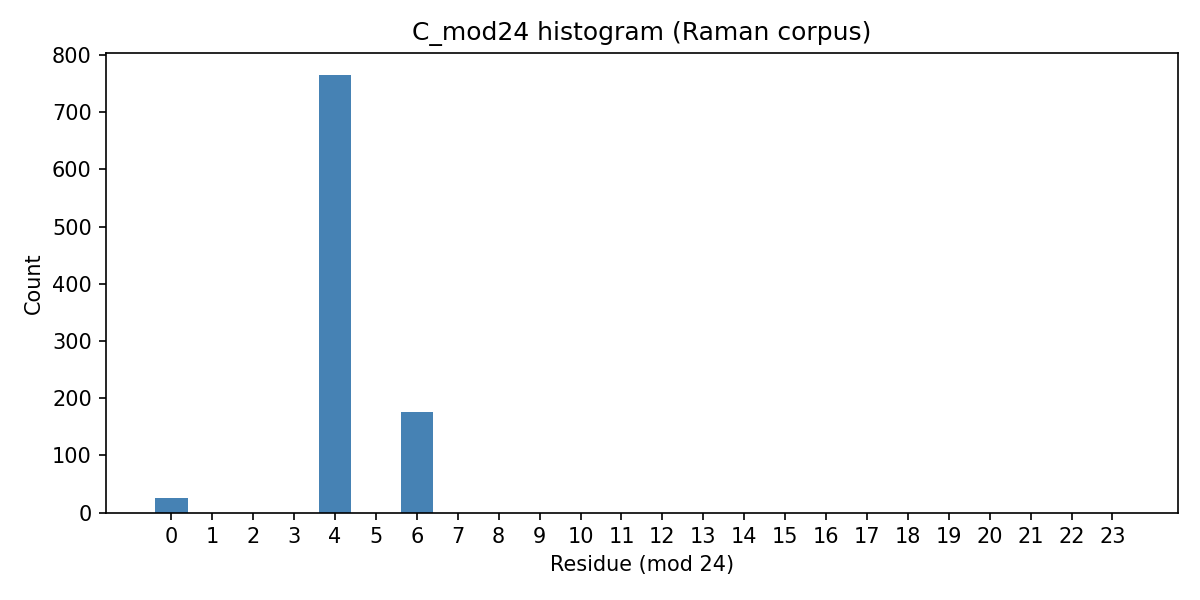
\includegraphics[width=0.85\linewidth]{figures/cm24_hist.png}
  \caption{C\textsubscript{mod 24} histogram.}
\end{figure}

\begin{figure}[H]
  \centering
  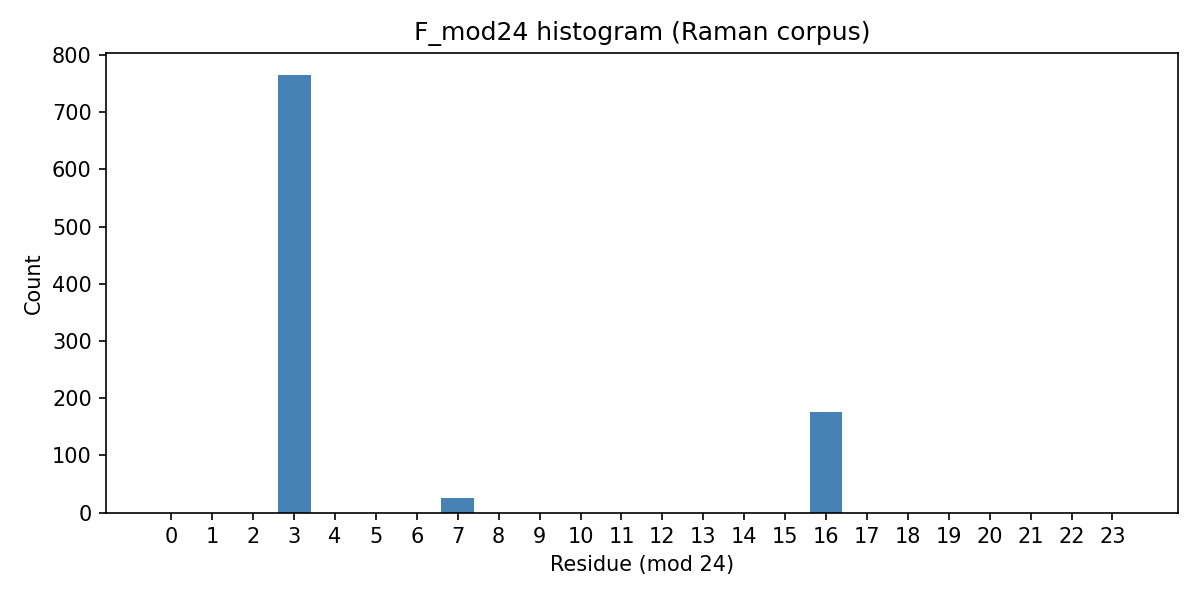
\includegraphics[width=0.85\linewidth]{figures/fm24_hist.png}
  \caption{F\textsubscript{mod 24} histogram.}
\end{figure}

\section*{SI-8: Reproducibility and CLI Commands}
All scripts are provided for end-to-end reproducibility:
\begin{itemize}
  \item Mapping: \texttt{python scripts/qa\_raman\_map\_files.py --roots qa\_data/raman data --labels ... --max-files 20000}
  \item Export features (Rust-backed invariants): \texttt{python scripts/qa\_raman\_features\_to\_csv.py --labels ... --modality Raman}
  \item Baselines: \texttt{python scripts/qa\_qafeature\_baseline.py --labels ...}, \texttt{python scripts/qa\_knn\_baseline.py --labels ... --k 5 --weighted}
  \item Ablations: \texttt{python scripts/qa\_feature\_ablation.py --labels ... --k 5 --save-csv --save-md}
  \item Report: \texttt{python scripts/qa\_benchmark\_report.py --labels ... --k 5}
  \item k-sweep: \texttt{python scripts/qa\_knn\_sweep.py --labels ... --k-list 1,3,5,7}
  \item Residue histograms: \texttt{python scripts/qa\_residue\_histograms.py}
\end{itemize}

Rust kernel health check:
\begin{verbatim}
python - << 'PY'
import importlib
qa = importlib.import_module('qa_lab_rs')
assert qa.ping() == 'qa_lab_rs:ok'
print('Rust QA kernel OK')
PY
\end{verbatim}

\end{document}

